\newpage
\section{Ergebnisse}
\label{sec:ergebnisse}

\subsection*{Messdaten}


\begin{table}[h!]
	\renewcommand*{\arraystretch}{1.2}
	\centering
	%\rowcolors{2}{white}{gray!25}
	\caption{Messdaten}
	\label{tab:messdaten}
	\resizebox{15cm}{!}{
		\begin{tabulary}{1.3\textwidth}{L|L|C|CCC|CC|C}
		\hline
		\textbf{Messdaten} & \multicolumn{2}{c|}{Messreihe}&\textbf{1}&\textbf{2}&\textbf{3}&\textbf{4}&\textbf{5}&\textbf{6}\\
		\hline
		&Kompressorleistung& \syein{P}{\watt}&360&380&410&400&380&400\\
		\hline
		& Umgebungsdruck& \syein{p_u}{\kilo \pascal}&\multicolumn{6}{c}{101,7}\\
		\hline
		\multirow{10}{*}{R134a}	&Massenstrom Kältemittel		&\syein{\dot{m}_{KM}}{\gram \per \second}&5,0&5,8&6,5&6,1&5,7&6,0\\
														&gemessener Verdampferdruck&\syein{\text{d}p_1}{\kilo \pascal}&115&140&180&155&120&160\\
														&absoluter Verdampferdruck		&\syein{p_1}{\kilo \pascal}&216,7&241,7&281,7&256,7&221,7&261,7\\
														&gemessener Kondensatordruck	&\syein{\text{d}p_2}{\kilo \pascal}&600&720&1900&870&800&803\\
														&absoluter Kondensatordruck			&\syein{p_2}{\kilo \pascal}&701,7&821,7&2001,7&971,7&901,7&904,7\\
														&Verdampferaustrittstemperatur	&\syein{t_1}{\celsius}&8,4&8,1&7,8&7,8&10,2&14,4\\
														&Kondensatoreintritts- temperatur	&\syein{t_2}{\celsius}&60,0&64,3&67,7&67,8&56,4&65,2\\
														&Kondensatoraustritts- temperatur	&\syein{t_3}{\celsius}&21,9&26,0&34,0&33,2&30,6&32,8\\
														&Verdampfereintrittstemperatur	&\syein{t_4}{\celsius}&-9,5&-6,1&-3,8&-4,8&-8,4&-2,7\\
		\hline
		\multirow{3}{*}{\shortstack{Kompressor- \\ kühlung}} & Massenstrom Kühlwasser & \syein{\dot{m}_{KW}}{\gram \per \second}&27&20&15&15&15&16\\
																&Eintrittstemperatur Kühlwasser&\syein{t_5}{\celsius}&7,7&7,6&7,8&7,7&7,8&8,3\\
																&Austrittstemperatur Kühlwasser&\syein{t_6}{\celsius}&8,2&8,7&9,3&9,3&8,9&9,6\\
		\hline
		\multirow{3}{*}{\shortstack{Kondensator-\\kühlung}} & Massenstrom Kühlwasser & \syein{\dot{m}_{KW}}{\gram \per \second}&27&20&15&15&15&16\\
																&Eintrittstemperatur Kühlwasser&\syein{t_6}{\celsius}&8,2&8,7&9,3&9,3&8,9&9,6\\
																&Austrittstemperatur Kühlwasser&\syein{t_7}{\celsius}&19,8&26,5&34,0&32,1&29,7&32,6\\
		\hline
		\multirow{3}{*}{\shortstack{wasser- \\durchströmter\\ Verdampfer}} & Massenstrom Kühlwasser & \syein{\dot{m}_{KW}}{\gram \per \second}&50&50&50&35&20&-\\
																&Eintrittstemperatur Kühlwasser&\syein{t_5}{\celsius}&7,7&7,6&7,8&7,7&7,8&-\\
																&Austrittstemperatur Kühlwasser&\syein{t_8}{\celsius}&3,1&3,0&2,6&1,0&0&-\\
			\hline
		\end{tabulary}
}
\end{table}%
\FloatBarrier

% Table generated by Excel2LaTeX from sheet 'Daten'
\begin{table}[h!]
	\renewcommand*{\arraystretch}{1.2}
	\centering
	%\rowcolors{2}{white}{gray!25}
	\caption{Messdaten zu Messreihe 6 - luftgekoppelter Verdampfer}
	\label{tab:mess_luft}
	\resizebox{\textwidth}{!}{
		\begin{tabulary}{1.1\textwidth}{L|C|CCCCC|C}
			\hline
			\multicolumn{2}{c|}{\textbf{Messpunkt}}&\textbf{1}&\textbf{2}&\textbf{3}&\textbf{4}&\textbf{5}&\textbf{Mittelwert}\\
			\hline
			\textbf{Luftaustrittsfläche}  &\syein{A}{\smeter}&\multicolumn{6}{c}{0,081}\\
			\hline
			\textbf{Umgebungstemperatur} &\syein{t_9}{\celsius}&\multicolumn{6}{c}{22,7}\\
			\hline
			\textbf{Luftaustrittstemperatur} &\syein{t_{10}}{\celsius}&5,3&9,2&4,9&9,4&16,2&9,0\\
			\hline
			\textbf{Luftgeschwindigkeit}&\syein{v}{\meter\per \second}&2,70&2,20&2,18&2,43&1,84&2,27\\
			\hline
	\end{tabulary}
}
\end{table}%
\FloatBarrier

\newpage

\subsection*{Auswertung der Messdaten}
Die Auswertung der aufgenommenen Messreihen beginnt bei \mbox{Messreihe 6}, da hier aufgrund des luftgekoppelten Verdampfers zusätzliche Auswertungsschritte notwendig sind.\\
Wie in Tabelle \ref{tab:zusatz_m6} festgehalten, wird angenommen, dass die Wärmekapazität, sowie die Dichte der Luft mit den dargestellten Werten als konstant angenommen werden.\\
Die Berechnung des Volumenstroms sowie des Massenstrom der Luft sind in den Gleichungen \ref{gl:volumenstrom} und \ref{gl:massenstrom} dargestellt. \\
Folgende Berechnungen, wie die der übertragenen Wärmen, werden sich auf die Mittelwerte und Annahmen dieser Tabelle \ref{tab:zusatz_m6} beziehen.

\begin{flalign}
	\label{gl:volumenstrom}
	\dot{V}_{L} &= v_{L} *A = \SI{2,70}{\meter \per \second}*\SI{0,081}{\smeter}\\
								&= \underline{\pyr[2]{2.7*0.081}{\kmeter \per \second}}
\end{flalign}

\begin{flalign}
	\label{gl:massenstrom}
	\dot{m}_{L} &= \dot{V}_{L} *\rho_L = \pyr[2]{2.7*0.081}{\kmeter \per \second}*\SI{1,2}{\kg \per \kmeter}\\
	&=\underline{ \pyr[2]{2.7*0.081*1.2}{\kg \per \second}}
\end{flalign}

% Table generated by Excel2LaTeX from sheet 'Daten'
\begin{table}[h!]
	\renewcommand*{\arraystretch}{1.2}
	\centering
	%\rowcolors{2}{white}{gray!25}
	\caption{zusätzliche Auswertung von Messreihe 6}
	\label{tab:zusatz_m6}
	\resizebox{\textwidth}{!}{
	\begin{tabulary}{1.1\textwidth}{L|C|CCCCC|C}
		\hline
		\multicolumn{2}{c|}{\textbf{Messpunkt}}&\textbf{1}&\textbf{2}&\textbf{3}&\textbf{4}&\textbf{5}&\textbf{Mittelwert}\\
		\hline
		\textbf{Dichte der Luft} &\syein{\rho_L}{\kg \per \kmeter}&\multicolumn{6}{c}{1,2}\\
		\hline
			\textbf{Wärmekapazität der Luft}&\syein{c_{p_{L}}}{\kilo \joule \per \kilo \gram \per \kelvin}&\multicolumn{6}{c}{1,0}\\
		\hline
			\textbf{Volumenstrom der Luft}  &\syein{\dot{V}_L}{\kmeter \per \second}&0,22&0,18&0,18&0,20&0,15&0,18\\
		\textbf{Massenstrom der Luft} &\syein{\dot{m}_L}{\kg \per \second}&0,26&0,22&0,22&0,24&0,18&0,22\\
		\hline
	\end{tabulary}
	}
\end{table}%
\FloatBarrier

Es folgen die Berechnungen zu Tab. \ref{tab:auswertung} und Tab. \ref{tab:auf4_5_7}. Innerhalb dieser Gleichungen sind ebenfalls die geforderten Lösungen der Aufgaben aufgeführt.
Die maßgebliche Grundgleichung für die Berechnungen der Wärmen ist unter \eqref{gl:ggl} zu finden.
\begin{flalign}
	\label{gl:ggl}
	\dot{Q} &= \dot{m}*c_p*\Delta T = \dot{m}*\left(h_i-h_j\right)
\end{flalign}

\newpage

\subsection*{Berechnungen zu Tabelle \ref{tab:auswertung}}

\begin{flalign}
	P_{\text{Dia}} &= \dot{m}_{KM}*\left(h_2-h_1\right)= \SI{5,0e-3}{\kg \per \second}*\left(\SI{446}{\kilo \joule \per \kg}-\SI{408}{\kilo \joule \per \kg}\right)\\
	&=\underline{\pyr{5*(446-408)}{\watt}}
\end{flalign}
\vspace{-10mm}

\begin{flalign}
	\dot{V}_1 &= v_1*\dot{m}_{KM} = \SI{30e-3}{\kmeter \per \kg}*\SI{5,0e-3}{\kg \per \second}\\
						&=\underline{\SI{1,5e-4}{\kmeter \per \second}}
\end{flalign}

\textbf{$\rightarrow$ entspricht Aufgabe 3 (Messreihe 1 bis  5):}
\begin{flalign}
	\dot{Q}_{\text{W,Verd}} 	
	&= \dot{m}_{KW, \text{Verdampfer}}*c_{P, \ce{H2O}}*\left(t_5-t_8\right)\\
	&= \SI{50e-3}{\kilo \gram \per \second}*\SI{4180}{\joule \per \kelvin \per \kilogram}*\left(7,7-3,1\right) \, \si{\kelvin}= \underline{\pyr{50*4.18*(7.7-3.1)}{\watt}}
\end{flalign}


\textbf{$\rightarrow$ entspricht Aufgabe 3 (Messreihe 6):}
\begin{flalign}
	\dot{Q}_{\text{L,Verd}} 	
	&= \dot{m}_{L}*c_{P, \text{Luft}}*\left(t_9-t_{10}\right)\\
	&= \SI{0,22e-3}{\kilo \gram \per \second}*\SI{1000}{\joule \per \kelvin \per \kilogram}*\left(22,7-9,0\right) \, \si{\kelvin}= \underline{\pyr{0.22*1*(22.7-9)}{\watt}}
\end{flalign}

\begin{flalign}
	\dot{Q}_{4-1} 
	&= \dot{m}_{KM}*\left(h_1-h_4\right)\\
	&= \SI{5,0e-3}{\kg \per \second}*\left(\SI{408e3}{\joule\per \kg}-\SI{230e3}{\joule\per \kg}\right)= \underline{\pyr{5/1000*(408*1000-230*1000)}{\watt}}
\end{flalign}

\textbf{$\rightarrow$ entspricht Aufgabe 2:}
\begin{flalign}
	\dot{Q}_{2-3} 
	&= \dot{m}_{KM}*\left(h_2-h_3\right)\\
	&= \SI{5,0e-3}{\kg \per \second}*\left(\SI{446e3}{\joule\per \kg}-\SI{230e3}{\joule\per \kg}\right)= \underline{\pyr{5/1000*(446*1000-230*1000)}{\watt}}
\end{flalign}

\begin{flalign}
	\dot{Q}_{\text{W, Kond}} 
	&= \dot{m}_{KW, \text{Kondensator}}*\left(t_7-t_6\right)\\
	&= \SI{27e-3}{\kg \per \second}*\SI{4,18}{\joule \per\kg \per \kelvin}*\left(19,8-8,2\right)\, \si{\kelvin}= \underline{\pyr{27*4.18*(19.8-8.2)}{\watt}}
\end{flalign}
\textit{$\rightarrow$ entspricht $\dot{Q}_H$}

\textbf{$\rightarrow$ entspricht Aufgabe 1:}
\begin{flalign}
	\dot{Q}_{1-2}
	&= \dot{m}_{KM}*\left(h_2-h_1\right)\\
	&= \SI{5,0e-3}{\kg \per \second}*\left(\SI{446e3}{\joule\per \kg}-\SI{408e3}{\joule\per \kg}\right) = \underline{\pyr{5/1000*(446*1000-408*1000)}{\watt}}
\end{flalign}

\begin{flalign}
	\dot{Q}_{\text{W, 5-6}} 
	&= \dot{m}_{KW, \text{Kompressor}}*\left(t_6-t_5\right)\\
	&= \SI{27e-3}{\kg \per \second}*\SI{4,18}{\joule \per\kg \per \kelvin}*\left(8,2-7,7\right)\, \si{\kelvin}= \underline{\pyr{27*4.18*(8.2-7.7)}{\watt}}
\end{flalign}
\begin{flalign}
	\dot{Q}_{\text{W, 5-7}} 
	&= \dot{m}_{KW, \text{Kompressor/Kondensator}}*\left(t_7-t_5\right)\\
	&= \SI{27e-3}{\kg \per \second}*\SI{4,18}{\joule \per\kg \per \kelvin}*\left(19,8-7,7\right)\, \si{\kelvin}= \underline{\pyr{27*4.18*(19.8-7.7)}{\watt}}
\end{flalign}

\textbf{$\rightarrow$ entspricht Aufgabe 4:}
\begin{flalign}
	\varepsilon &= \frac{\dot{Q}_{\text{W, Kond}} }{P} = \frac{\SI{1309}{\watt}}{\SI{360}{\watt}} =\underline{\pyr[1]{1309/360}{}}
\end{flalign}



\begin{flalign}
\pi &= \frac{p_2}{p_1}=\frac{\SI{701,7}{\kilo \pascal}}{\SI{216,7}{\kilo \pascal}} =\underline{\pyr[1]{701.7/216.7}{}}
\end{flalign}

\subsection*{Berechnungen zu Tabelle \ref{tab:auf4_5_7}}
\textbf{$\rightarrow$ entspricht Aufgabe 5:}
\begin{flalign}
	\varepsilon_{\text{Kond+Komp}} &= \frac{\dot{Q}_{\text{W, 5-7}} }{P} = \frac{\SI{1366}{\watt}}{\SI{360}{\watt}}\\
	&= \underline{\pyr[1]{1366/360}{}}
\end{flalign}

\textbf{$\rightarrow$ entspricht Aufgabe 7:}
\begin{flalign}
	\varepsilon_{\text{Kältemaschine}} &= \frac{\dot{Q}_{\text{W/L, Verd}} }{P} = \frac{\SI{961}{\watt}}{\SI{360}{\watt}}\\
	&= \underline{\pyr[1]{961/360}{}}
\end{flalign}


\begin{table}[h!]
	\renewcommand*{\arraystretch}{1.2}
	\centering
	%\rowcolors{2}{white}{gray!25}
	\caption{Ausgewertete Messdaten der Messreihe 1 bis 6}
	\label{tab:auswertung}
	\resizebox{\textwidth}{!}{
		\begin{tabulary}{1.3\textwidth}{L|C|CCC|CC|C}
			\hline
			 \multicolumn{2}{c|}{Messreihe}&\textbf{1}&\textbf{2}&\textbf{3}&\textbf{4}&\textbf{5}&\textbf{6}\\
			\hline
			Kompressorleistung&\syein{P}{\watt}&360&380&410&400&390&400\\
			Kompressorleistung (Dia)&\syein{P_{\text{Dia}}}{\watt}&190&220&163&336&114&264\\
			\hline
			\multirow{4}{*}{Kältemittelenthalpien} &\syein{h_1}{\kilo \joule \per \kg}&408&407&405&405&410&405\\
			&\syein{h_2}{\kilo \joule \per \kg}&446&445&430&460&430&449\\
			&\syein{h_3}{\kilo \joule \per \kg}&230&233&248&249&243&249\\
			&\syein{h_4}{\kilo \joule \per \kg}&230&233&248&249&243&249\\
			\hline
			Verdampfungstemperatur & \syein{t_4}{\celsius}&-9,5&-6,1&-3,8&-4,8&-8,4&-2,7\\
			\hline
			Kondensationstemperatur bei $p_2$ & \syein{t_{\text{Kond}}}{\celsius}&27&35&68&38&36&36\\
			\hline
			spezifisches Volumen &\syein{v_1}{ \raiseto{3} \deci \meter \per \kg}&30&25&9&21&23&78\\
			\hline
			Volumenstrom durch den Kompressor & \syein{\dot{V}_1*10^{-4}}{\kmeter \per \second}&1,5&1,5&0,59&1,3&1,3&4,7\\
			\hline
			Kältemittelmassenstrom &\syein{\dot{m}_{KM}*10^{-3}}{\kg \per \second}&5,0&5,8&6,5&6,1&5,7&6,0\\
			\hline
			Wärmeübertragung im Verdampfer &&&&&&&\\
			\textit{vom Wasser/Luft}& \syein{\dot{Q}_{\text{W, Verd}}}{\watt}&961&\textcolor{red}{961}&1087&980&\textcolor{red}{652}&3002\\
			\textit{an das Kältemittel }& \syein{\dot{Q}_{4-1}}{\watt}&890&\textcolor{red}{1009}&1021&952&\textcolor{red}{952}&936\\
			\hline
			Wärmeübertragung im Kondensator &&&&&&&\\
			\textit{vom Kältemittel }& \syein{\dot{Q}_{2-3}}{\watt}&\textcolor{red}{1080}&\textcolor{red}{1230}&\textcolor{red}{1183}&\textcolor{red}{1287}&\textcolor{red}{1066}&\textcolor{red}{1200}\\
			\textit{an das Wasser} & \syein{\dot{Q}_{\text{W, kond}}}{\watt}&\textcolor{red}{1309}&\textcolor{red}{1488}&\textcolor{red}{1549}&\textcolor{red}{1492}&\textcolor{red}{1304}&\textcolor{red}{1538}\\
			\hline
			Wärmeübertragung im Kompressor &&&&&&&\\
			\textit{vom Kältemittel} & \syein{\dot{Q}_{1-2}}{\watt}&190&220&163&336&114&264\\
			\textit{an das Wasser }& \syein{\dot{Q}_{\text{W, 5-6}}}{\watt}&56&92&94&100&69&87\\
			\hline
			Gesamtwärmeübertragung an das Wasser&\syein{\dot{Q}_{\text{W, 5-7}}}{\watt}&1366&1580&1643&1593&1373&1625\\
			\hline
			Leistungsziffer &\syein{\varepsilon}{-}&3,6&3,9&3,8&3,7&3,3&3,8\\
			\hline
			Druckverhältnis&\syein{\pi}{-}&3,2&3,4&7,1&3,8&4,1&3,5\\
			\hline
			
	\end{tabulary}
}
\end{table}%
\FloatBarrier

% Table generated by Excel2LaTeX from sheet 'Daten'
\begin{table}[h!]
	\renewcommand*{\arraystretch}{1.2}
	\centering
	%\rowcolors{2}{white}{gray!25}
	\caption{Leistungsziffern: Kondensationswärme, Kondensations- und Kompressionswärme, Kältemaschine}
	\label{tab:auf4_5_7}
	%\resizebox{10.5cm}{!}{
		\begin{tabulary}{1.0\textwidth}{CL|CCCCCC}
			\hline
			\multicolumn{2}{c}{\textbf{Messreihe} }& \textbf{1} & \textbf{2}&\textbf{3}&\textbf{4}&\textbf{5}&\textbf{6}\\
			\hline
			Leistungsziffer &\syein{\varepsilon_{\text{Kond}}}{-}&3,6&3,9&3,8&3,7&3,3&3,8\\
			Leistungsziffer &\syein{\varepsilon_{\text{Kond+Komp}}}{-}&3,8&4,2&4,0&4,0&3,5&4,1\\
			Leistungsziffer& \syein{\varepsilon_{\text{Kältemaschine}}}{-}&2,7&2,5&2,7&2,5&1,7&\textbf{7,5}\\
			\hline			
	\end{tabulary}
%}
\end{table}%
\FloatBarrier

\newpage

\subsubsection*{Aufgabe 6}
\textbf{Temperaturhub:}
\begin{flalign}
	\Delta T &= \left|t_{\text{Kond}}-t_4\right|=  \left|-9,5-27\right|\, \si{\kelvin}\\
	&=\underline{\SI{36,5}{\kelvin}}
\end{flalign}

\textbf{Kondensationswärme:}
\begin{flalign}
	\dot{Q}_K &= \dot{m}_{KM}*\left(h_{2,0}-h_{3,0}\right)\\
	& =\SI{5,0e-3}{\kg \per \second}*\left(\SI{412e3}{\joule \per \kg}-\SI{236e3}{\joule \per \kg}\right) =\underline{\SI{880}{\watt}}
\end{flalign}

\textbf{Überhitzungswärme:}
\begin{flalign}
	\dot{Q}_{\text{Ü}} &= \dot{m}_{KM}*\left(h_1-h_{1,0}\right)\\
	&=\SI{5,0e-3}{\kg \per \second}*\left(\SI{408e3}{\joule \per \kg}-\SI{389e3}{\joule \per \kg}\right)=\underline{\SI{95}{\watt}}
\end{flalign}

% Table generated by Excel2LaTeX from sheet 'Daten'
\begin{table}[h!]
	\renewcommand*{\arraystretch}{1.2}
	\centering
	%\rowcolors{2}{white}{gray!25}
	\caption{Übersicht, der grafisch darzustellenden Größen}
	\label{tab:dias}
	\resizebox{\textwidth}{!}{
	\begin{tabulary}{1.1\textwidth}{LC|CCCCCC}
		\hline
		\multicolumn{2}{c}{\textbf{Messreihe} }& \textbf{1} & \textbf{2}&\textbf{3}&\textbf{4}&\textbf{5}&\textbf{6}\\
		\hline
		Temperaturhub &\syein{\Delta T}{\kelvin}&36,5&41,1&71,8&42,8&44,4&38,7\\
		KM-Enthalpie (ohne Überhitzung) &\syein{h_{1,0}}{\kilo \joule \per \kg}&389&394&392&392&390&392\\
		KM-Enthalpie (ohne Überhitzung)& \syein{h_{2,0}}{\kilo \joule \per \kg}&412&415&429&419&418&418\\
		KM-Enthalpie (ohne Unterkühlung)& \syein{h_{3,0}}{\kilo \joule \per \kg}&236&241&301&255&250&251\\
		Kondensationswärme& \syein{Q_{K}}{\kilo \joule \per \kg}&880&1009&832&1000&958&1002\\
		Überhitzungswärme& \syein{Q_{Ü}}{\kilo \joule \per \kg}&95&75&85&79&114&78\\
		Heizwärme& \syein{Q_{H}}{\kilo \joule \per \kg}&1309&1488&1549&1492&1304&1538\\
		Überhitzungstemperatur& \syein{t_{Ü}}{\celsius}&8,4&8,1&7,8&7,8&10,2&14,4\\
		\hline			
	\end{tabulary}
	}
\end{table}%
\FloatBarrier

\begin{figure}[h!]
	\centering
	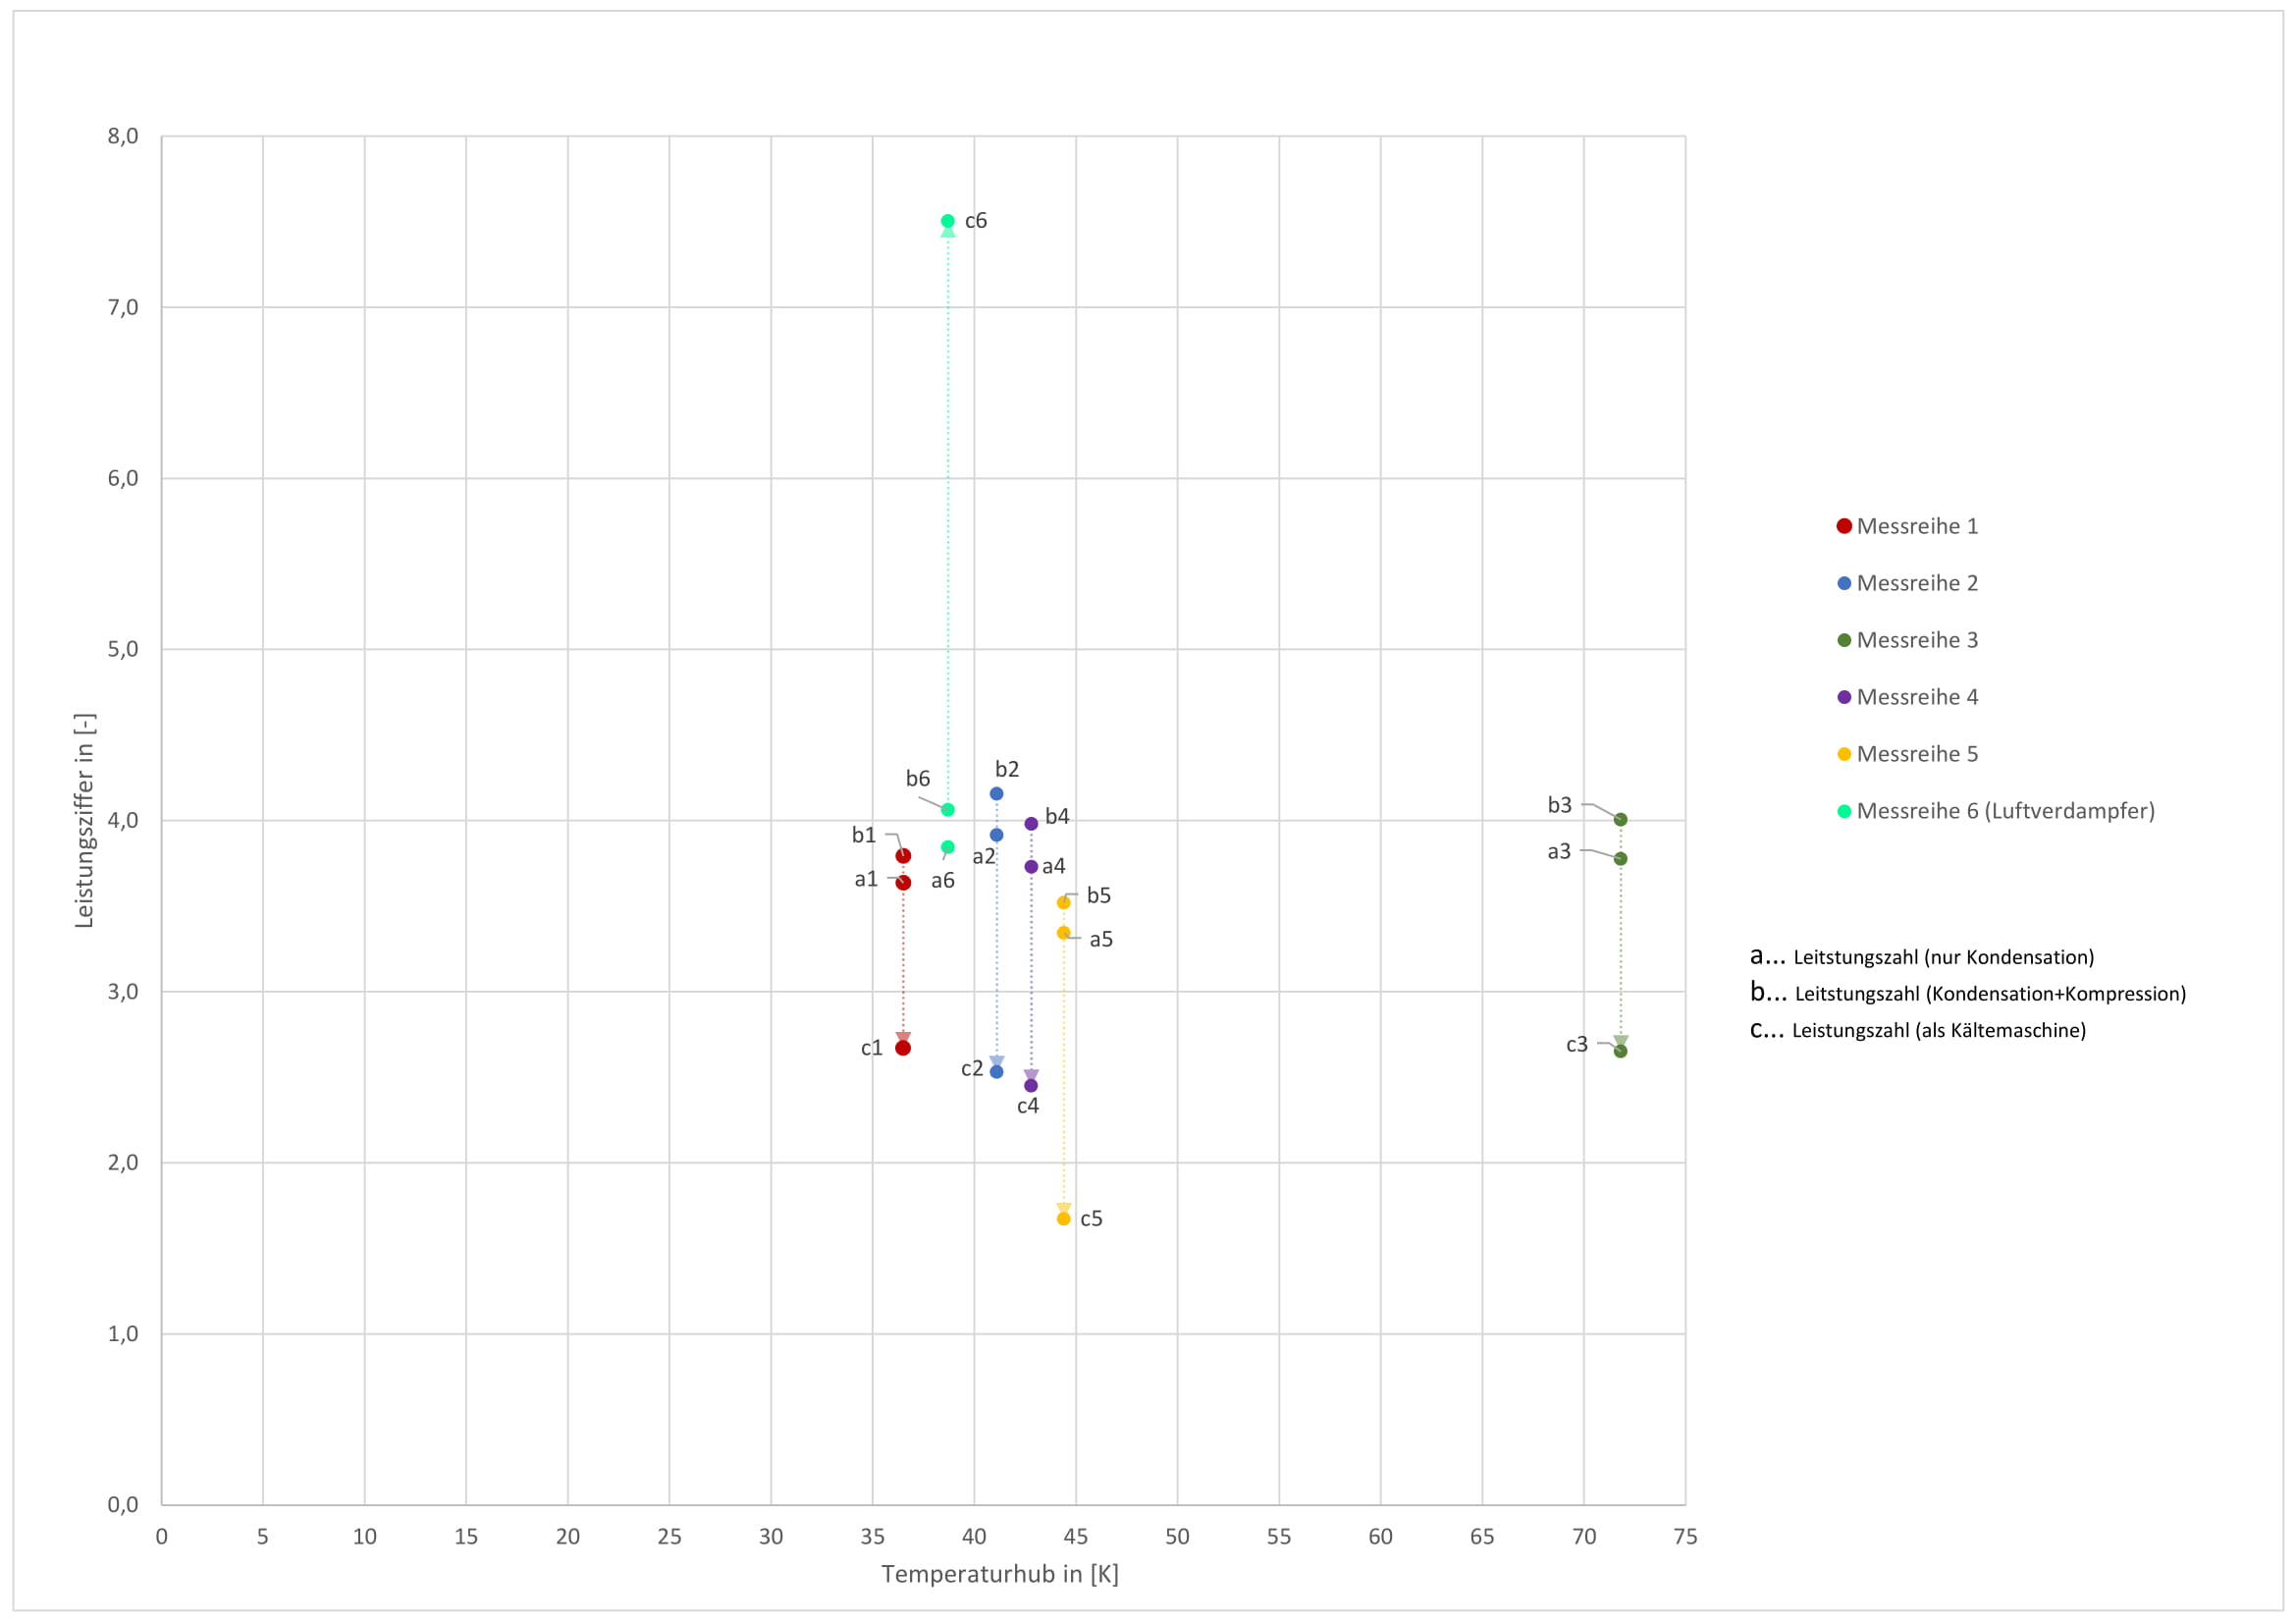
\includegraphics[width=1.0\textwidth]{img/diagramme-1}
	\caption{Leistungsziffern in Abhängigkeit vom Temperaturhub}
	\label{dia:lz_t}
\end{figure}
\FloatBarrier
%Ende
\begin{figure}[h!]
	\centering
	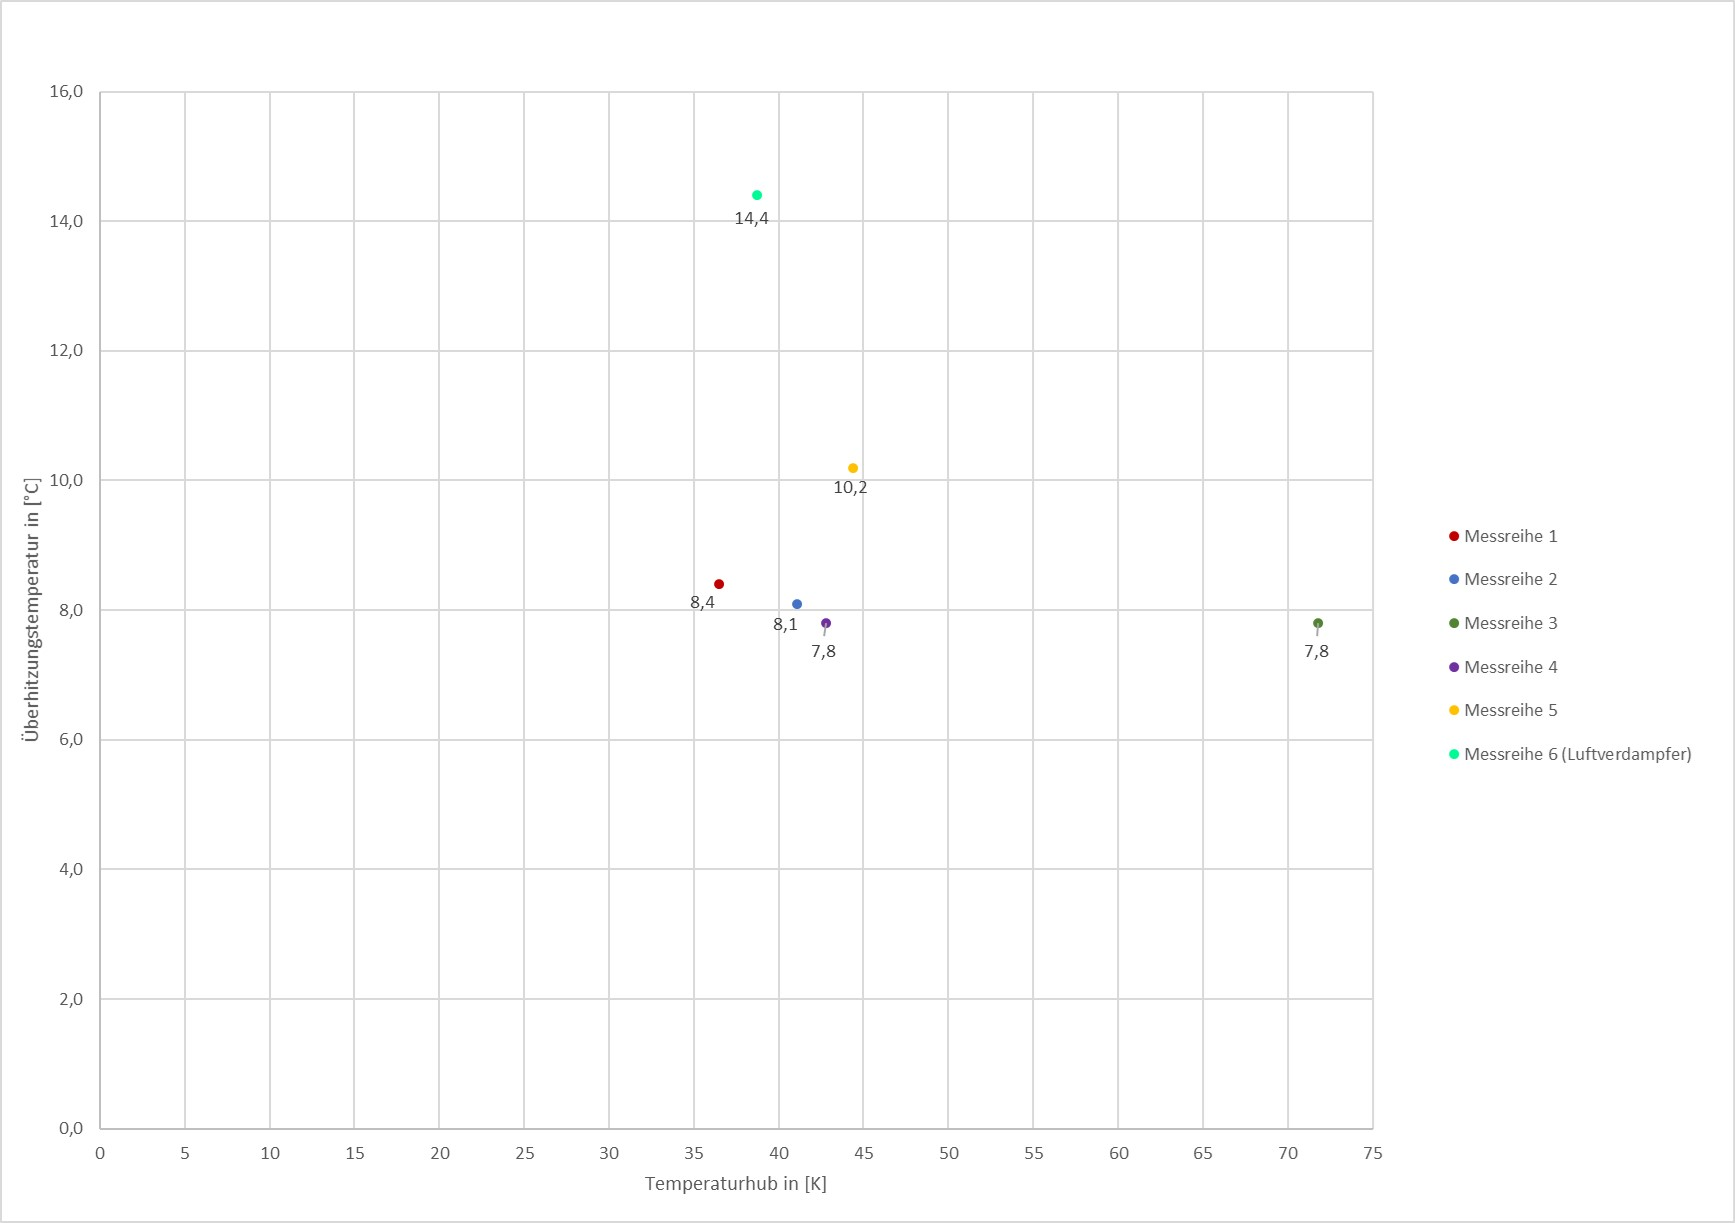
\includegraphics[width=1.0\textwidth]{img/diagramme-2}
	\caption{Überhitzungstemperaturen in Abhängigkeit vom Temperaturhub}
	\label{dia:tu_t}
\end{figure}
\FloatBarrier
%Ende
\begin{figure}[h!]
	\centering
	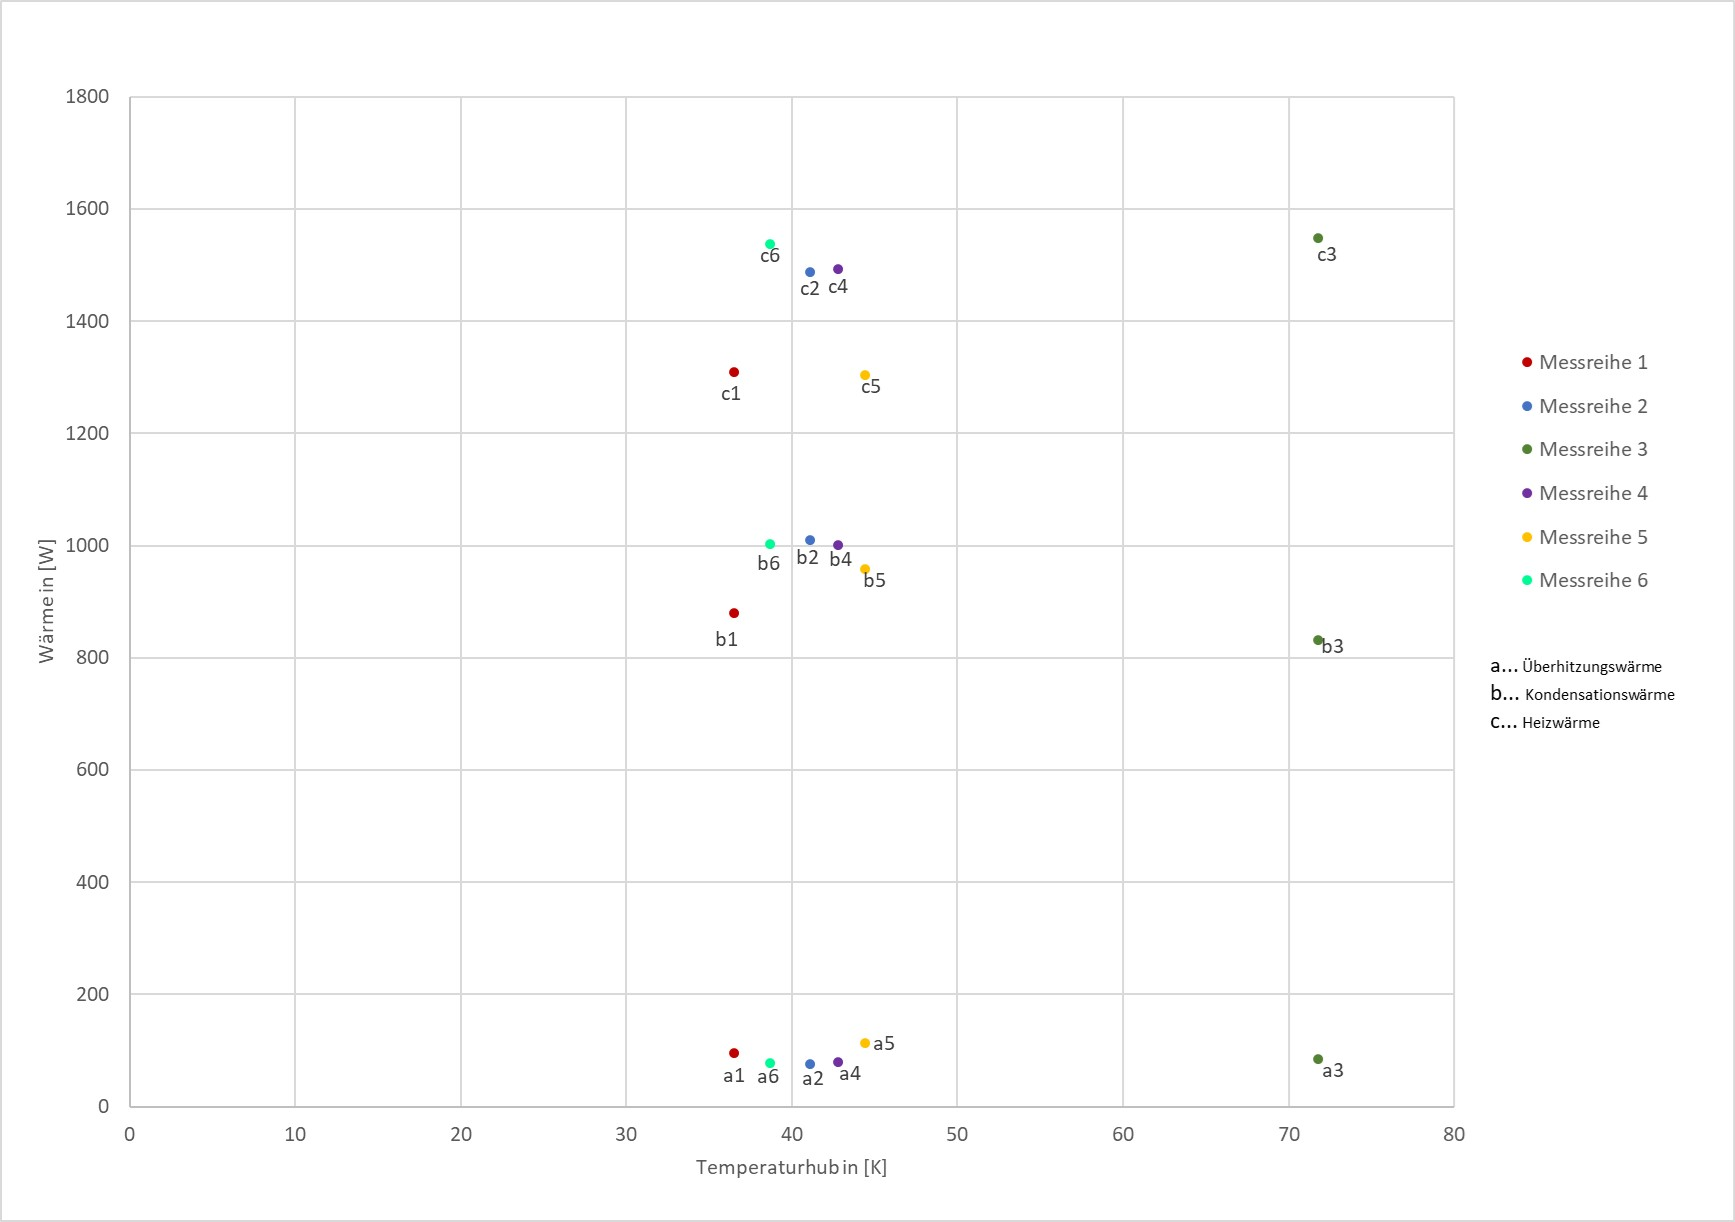
\includegraphics[width=1.0\textwidth]{img/diagramme-3}
	\caption{Überhitzungs-, Kondensations- und Heizwärme in Abhängigkeit vom Temperaturhub}
	\label{dia:q_t}
\end{figure}
\FloatBarrier
%Ende

